\section{ArXe-Clusters}
In heteronuclear ArXe clusters \ac{ICD} and \ac{ETMD}3 are theoretically
possible after creation of an Ar3s vacancy. The final states of these processes
are characterized by Ar3p$^{-1}$Xe5p$^{-1}$ and Xe5p$^{-1}$Xe5p$^{-1}$,
respectively. As discussed in section \ref{section:icd_geom}, all \ac{ICD}
for distances shorther than \unit[10]{\AA}. From this perspective the
slower \ac{ETMD}3, but at equilibrium geometries
of the ArXe$_2$ trimer energetically accessible process should be
observable in experiment \cite{Fasshauer10}. 

In the following first the basic cluster and spin-orbit coupling effects
are investigated using easiest model
structures. Afterwards, cluster structures investigated and compared to experiment.


\subsection{Model structures}
In order to model the decay processes in clusters an Ausschnitt of an cluster
is modelled by layers of xenon atoms in an \ac{fcc} structure. On these
layers, one argon atom is placed in either a \ac{fcc} or an \ac{hcp} position
as shown in figure \ref{figure:model_clusters}. The atomic distance are
assumed to equal the sum of the corresponding van der Waals radii given in
table \ref{table:vdWaalsradii}.

\begin{figure}[htb]
 \centering
 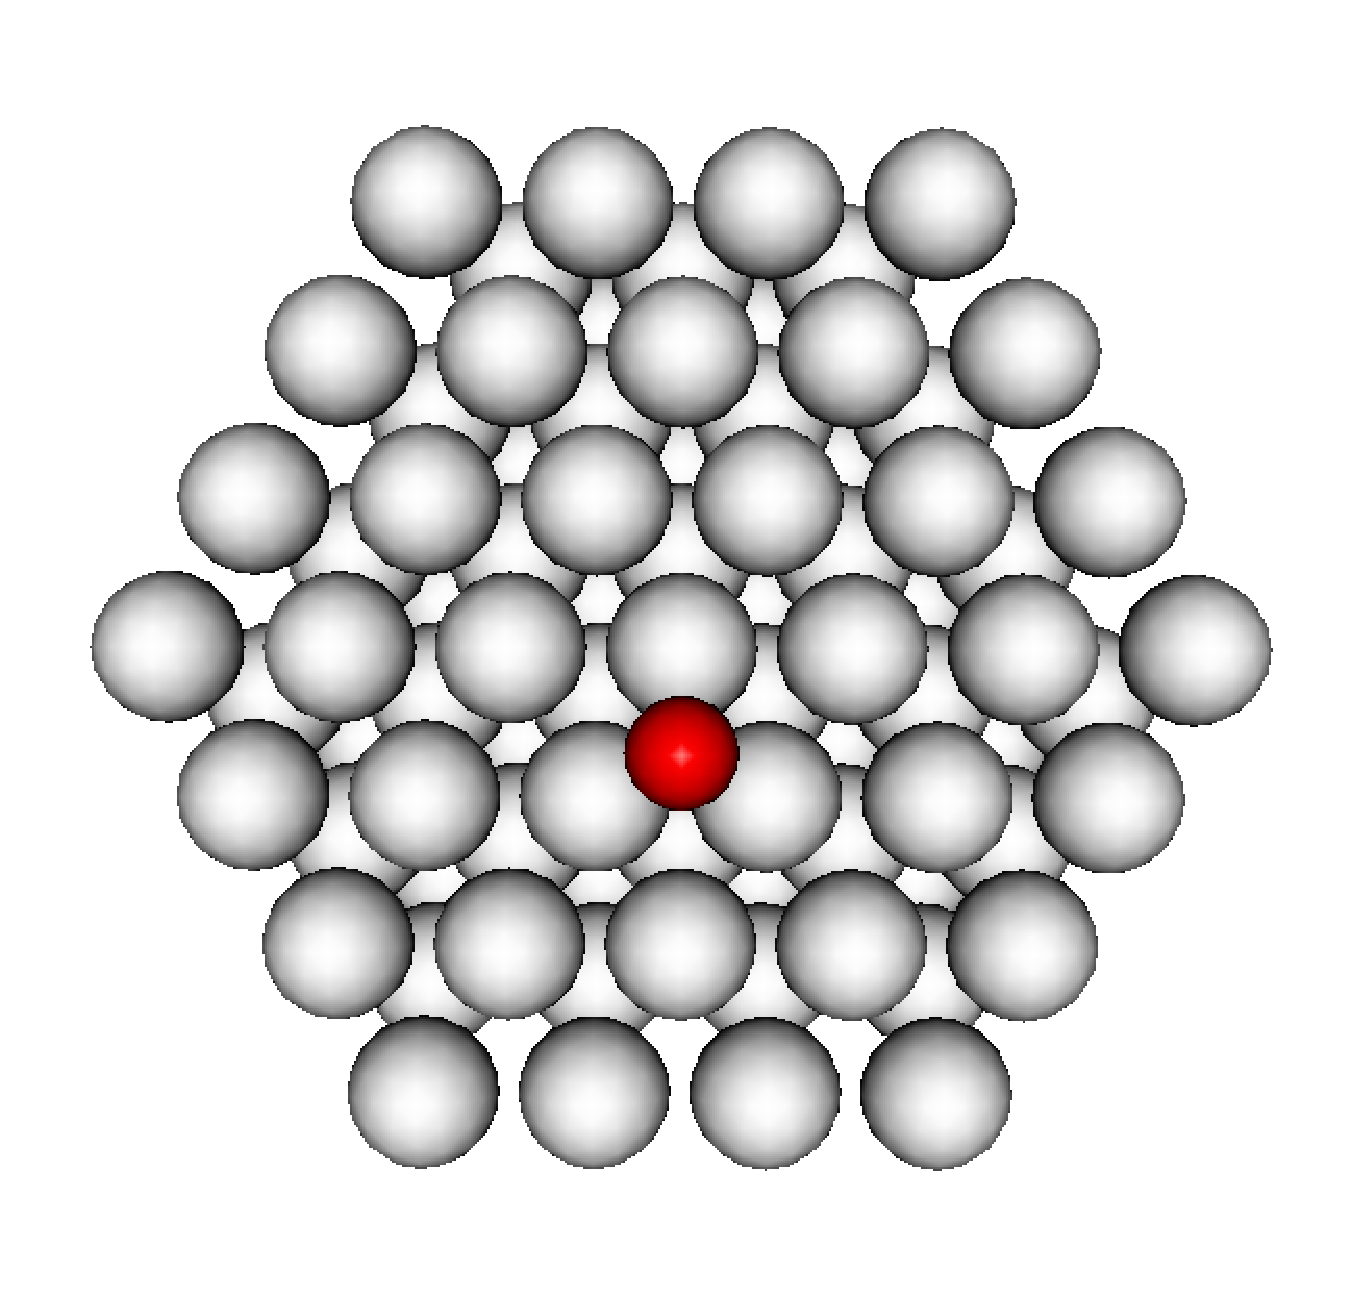
\includegraphics[scale=0.27]{pics/fcc.eps}
 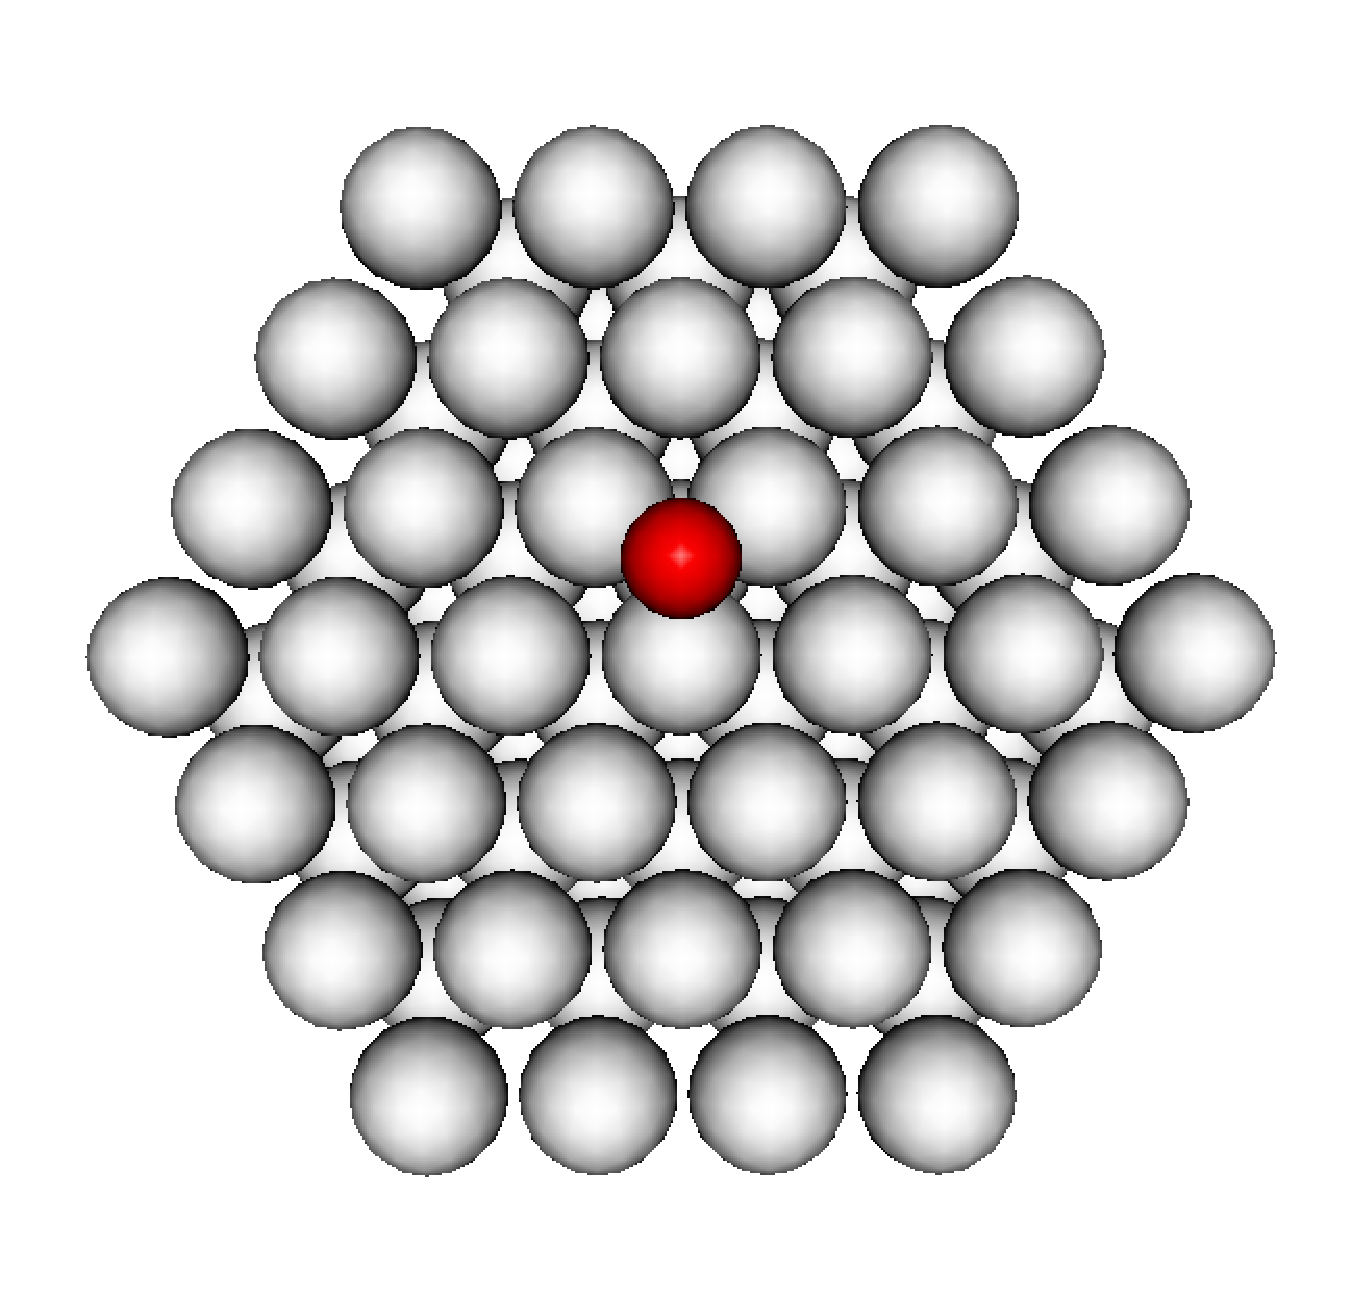
\includegraphics[scale=0.27]{pics/hcp.eps}
 \caption{Model structures of ArXe clusters.\\
          Left panel: Argon atom placed
          in an \ac{fcc} position on xenon atom layers in \ac{fcc} structure.\\
          Right panel: Argon atom placed
          in an \ac{fcc} position on xenon atom layers in \ac{fcc} structure.}
 \label{figure:model_clusters}
\end{figure}

The initial and final state energies are estimated by shifted atomic
ionization energies.
Since atoms in clusters interact with each other and especially
charges are stabilized in noble gas clusters, the atomic
ionization energies  in table \ref{table:noble_atom_ionization} alone
are no good approximation. In order to take care of
this stabilization effect, the ionization energies are corrected by experimentally
observed shifts between atomic and cluster ionization energies of homonuclear
clusters given in table
\ref{table:cluster_shifts} in the appendix. These shifts do account for
higher or
lower charge stabilization by other neighbouring atoms of other elements.

From these shifted ionization energies other potential curves of initial and
final states are achieved shown in figure \ref{ArXe_energy_curves_shifted}.

\begin{figure}[htb]
 \centering
 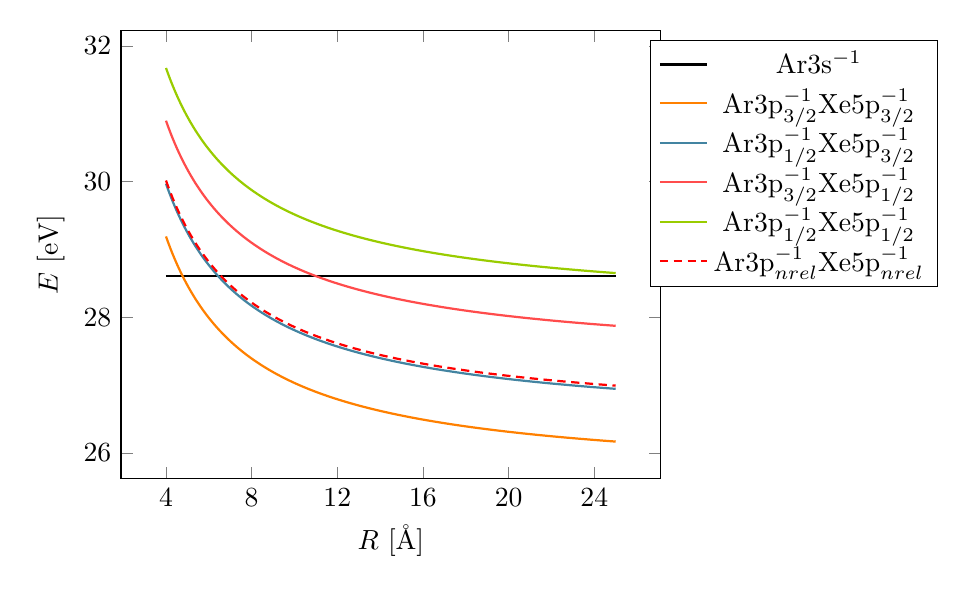
\begin{tikzpicture}
    \begin{axis}[domain=4.0:25,
                 samples = 200,
                 xtick={4.0,8.0,...,24},
                 %xticklabels={$-\pi$,$-\frac \pi 2$,0,$\frac \pi 2$,$\pi$},
                 cycle list name = exotic,
                 legend style={anchor= north west},
                 xlabel={$R$ [\AA]},
                 ylabel={$E$ [eV]}
                 ]
      \addplot+[
                mark = none,
                black,
                thick
               ]
               {29.239 - 0.636};
      \addlegendentry{Ar3s$^{-1}$};
      \addplot+[
                mark = none,
                thick
               ]
               {15.7596 - 1.0 + 12.1298 - 1.3 + 14.39964 / x};
      \addlegendentry{Ar3p$_{3/2}^{-1}$Xe5p$_{3/2}^{-1}$};
      \addplot+[
                mark = none,
                thick
               ]
               {15.9371 - 0.4 + 12.1298 -1.3 + 14.39964 / x};
      \addlegendentry{Ar3p$_{1/2}^{-1}$Xe5p$_{3/2}^{-1}$};
      \addplot+[
                mark = none,
                thick
               ]
               {15.7596 - 1.0 + 13.4363 -0.9 + 14.39964 / x};
      \addlegendentry{Ar3p$_{3/2}^{-1}$Xe5p$_{1/2}^{-1}$};
      \addplot+[
                mark = none,
                thick
               ]
               {15.9371 -0.4 + 13.4363 - 0.9 + 14.39964 / x};
      \addlegendentry{Ar3p$_{1/2}^{-1}$Xe5p$_{1/2}^{-1}$};
      \addplot+[
                mark = none,
                thick
               ]
               {15.8188 - 0.8 + 12.5653 - 1.17 + 14.39964 / x};
      \addlegendentry{Ar3p$_{nrel}^{-1}$Xe5p$_{nrel}^{-1}$};
      %\draw[] (axis cs:\pgfkeysvalueof{/pgfplots/xmin},29.239) -- (axis cs:\pgfkeysvalueof{/pgfplots/xmax},29.239);
    \end{axis}
\end{tikzpicture}

 \caption{Initial and final state energies of the ICD channels of ArXe in the
          model of pairs calculated from shifted atomic ionization energies.
          Both the four relativistic channels and
          the non-relativistic estimate are shown. From the distance on, where
          the final state energy is lower than the initial state energy, the
          decay channel is open.}
 \label{ArXe_energy_curves_shifted}
\end{figure}

Compared to the results using unshifted ionization energies of section
\ref{section_icd_geom} the
channel opening distances are shorter.
In detail they are \unit[4.78]{\AA}, \unit[6.44]{\AA}, \unit[11.02]{\AA}
and \unit[27.19]{\AA} for the Ar3p$_{3/2}^{-1}$Xe5p$_{3/2}^{-1}$,
Ar3p$_{1/2}^{-1}$Xe5p$_{3/2}^{-1}$, Ar3p$_{3/2}^{-1}$Xe5p$_{1/2}^{-1}$ and
Ar3p$_{1/2}^{-1}$Xe5p$_{1/2}^{-1}$ channel, respectively. The channel
opening distance in the Russel-Saunders coupling scheme is \unit[6.58]{\AA}.
This means that all \ac{ICD} channels are still closed at the equilibrium
distance of the ArXe dimer. But inside a cluster also larger distances are
to be found. Already for the next-nearest neighbours the
Ar3p$_{3/2}^{-1}$Xe5p$_{3/2}^{-1}$ channel is open. Hence, the \ac{ICD}
process can not be neglected in the further investigations.

The potential curves of the initial and final states of the \ac{ETMD}3
process are shown in figure \ref{figure:ArXe_energy_etmd_curves}, where
$R$ here denotes the distance between the two xenon atoms.

\begin{figure}[htb]
 \centering
 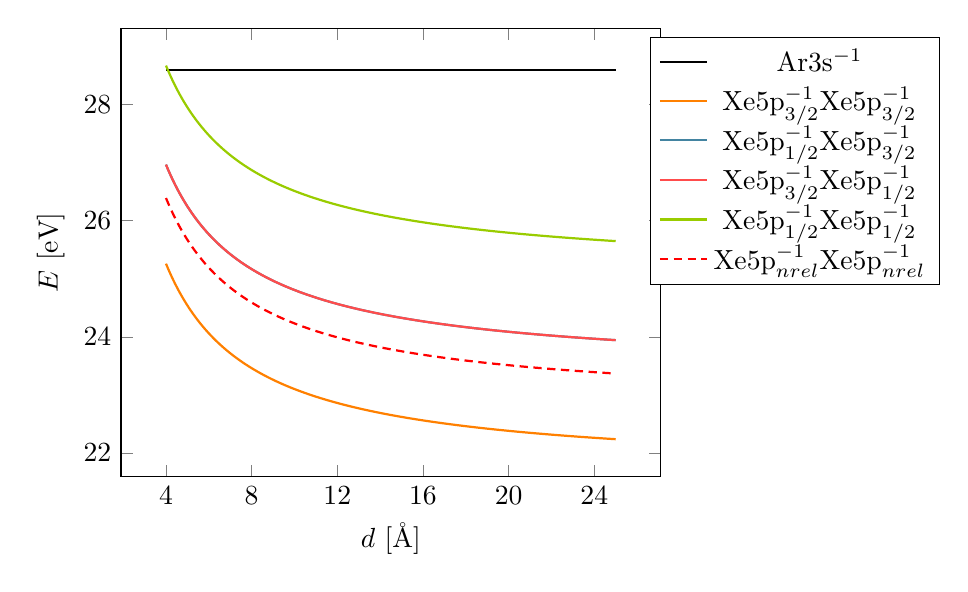
\begin{tikzpicture}
    \begin{axis}[domain=4.0:25,
                 samples = 200,
                 xtick={4.0,8.0,...,24},
                 %xticklabels={$-\pi$,$-\frac \pi 2$,0,$\frac \pi 2$,$\pi$},
                 cycle list name = exotic,
                 legend style={anchor= north west},
                 xlabel={$d$ [\AA]},
                 ylabel={$E$ [eV]}
                 ]
      \addplot+[
                mark = none,
                black,
                thick
               ]
               {29.239 - 0.636};
      \addlegendentry{Ar3s$^{-1}$};
      \addplot+[
                mark = none,
                thick
               ]
               {12.1298 - 1.3 + 12.1298 - 1.3 + 14.39964 / x};
      \addlegendentry{Xe5p$_{3/2}^{-1}$Xe5p$_{3/2}^{-1}$};
      \addplot+[
                mark = none,
                thick
               ]
               {13.4363 - 0.9 + 12.1298 -1.3 + 14.39964 / x};
      \addlegendentry{Xe5p$_{1/2}^{-1}$Xe5p$_{3/2}^{-1}$};
      \addplot+[
                mark = none,
                thick
               ]
               {12.1298 - 1.3 + 13.4363 -0.9 + 14.39964 / x};
      \addlegendentry{Xe5p$_{3/2}^{-1}$Xe5p$_{1/2}^{-1}$};
      \addplot+[
                mark = none,
                thick
               ]
               {13.4363 - 0.9 + 13.4363 - 0.9 + 14.39964 / x};
      \addlegendentry{Xe5p$_{1/2}^{-1}$Xe5p$_{1/2}^{-1}$};
      \addplot+[
                mark = none,
                thick
               ]
               {12.5653 - 1.17 + 12.5653 - 1.17 + 14.39964 / x};
      \addlegendentry{Xe5p$_{nrel}^{-1}$Xe5p$_{nrel}^{-1}$};

    \end{axis}
\end{tikzpicture}

 \caption{Initial and final state energies of the \ac{ETMD}3 channels
          in the model of triples calculated from shifted atomic ionization
          energies.}
 \label{figure:ArXe_energy_etmd_curves}
\end{figure}

The final state energies of the Xe5p$_{1/2}^{-1}$Xe5p$_{3/2}^{-1}$ and
the Xe5p$_{3/2}^{-1}$Xe5p$_{1/2}^{-1}$ are degenerate, but the channels
differ by the quantum
numbers of the vacancy filling an the emitted electron. Hence, the decay
widths are not necessarily equal and need to be treated separately.
For all distances larger than the equilibrium distance of \unit[4.04]{\AA}
all \ac{ETMD}3 channels are open. Therefore, the decay can occur with
nearest neighbours, which enable the highest possible decay width.

From the consideration of channel opening distances it is not clear, whether
either of the two competing processes is much faster and would hence dominate
an experimental spectrum. Another aspect of clusters is the multitude of
possible decay partners. For the \ac{ICD}, the number of decay partners equals
the number of xenon atoms $N_{Xe}$, while for the \ac{ETMD}3 process the number
of triples for each argon atoms is given by $N_{Xe}^2$. This means that
the \ac{ETMD}3 is statistically favoured above the \ac{ICD} in clusters with
xenon cores consisting of more than one xenon atom.

\begin{figure}[ht]
 \centering
 \begin{tikzpicture}[scale=1.0]

\begin{axis}[%scale=1.5,
             domain=0:7,
             restrict expr to domain={x}{0:7},
             %restrict expr to domain={y}{1.0E-12:7},
             xlabel={E [eV]},
             %xtick={30,50,...,170},
             %xticklabels={2,4,6,8,10,12,15,20,25},
             %ytick={-1.0,-0.8,...,1.0},
             %yticklabels={1.0,0.8,0.6,0.4,0.2,0.0,0.2,0.4,0.6,0.8,1.0},
             ylabel={$\Gamma$ [eV]},
             scale only axis,
             width=\textwidth-1.5cm,
             height=8cm,
             %ybar stacked
             ]

%ICD
\addplot+[ycomb,
         mark=.,
         very thick,
         diplom1,
         forget plot
        ]
        table[
        x expr = \thisrowno{0},
        y expr = \thisrowno{1}
        ]
        {data/arxe_model_icd_rel.dat};
        \addlegendimage{line legend, diplom1, very thick};
        \addlegendentry{ICD};

%ETMD
\addplot+[ycomb,
         mark=.,
         very thick,
         diplom2,
         forget plot
        ]
        table[
        x expr = \thisrowno{0},
        y expr = \thisrowno{1}
        ]
        {data/arxe_model_etmd_rel.dat};
        \addlegendimage{line legend, diplom2, very thick};
        \addlegendentry{ETMD};


%Folded
\addplot[
         mark=none,
         color=gray,
         dotted,
         thick
         ]
         table[
         x expr=\thisrowno{0},
         y expr=\thisrowno{1}
         ]
         {data/arxe_model_icd_rel.sp};
         \addlegendentry{ICD spectrum};

\addplot[
         mark=none,
         color=gray,
         dashed,
         thick
         ]
         table[
         x expr=\thisrowno{0},
         y expr=\thisrowno{1}
         ]
         {data/arxe_model_etmd_rel.sp};
         \addlegendentry{ETMD spectrum};

\addplot[
         mark=none,
         color=gray,
         thick
         ]
         table[
         x expr=\thisrowno{0},
         y expr=\thisrowno{1}
         ]
         {data/arxe_model_kombi_rel.sp};
         \addlegendentry{full spectrum};



\end{axis}
\end{tikzpicture}

 \begin{tikzpicture}[scale=1.0]

\begin{axis}[%scale=1.5,
             domain=0:7,
             restrict expr to domain={x}{0:7},
             %restrict expr to domain={y}{1.0E-12:7},
             xlabel={E [eV]},
             %xtick={30,50,...,170},
             %xticklabels={2,4,6,8,10,12,15,20,25},
             %ytick={-1.0,-0.8,...,1.0},
             %yticklabels={1.0,0.8,0.6,0.4,0.2,0.0,0.2,0.4,0.6,0.8,1.0},
             ylabel={$\Gamma$ [eV]},
             scale only axis,
             width=\textwidth-1.5cm,
             height=8cm,
             %ybar stacked
             ]

%ICD
\addplot+[ycomb,
         mark=.,
         very thick,
         diplom1,
         forget plot
        ]
        table[
        x expr = \thisrowno{0},
        y expr = \thisrowno{1}
        ]
        {data/arxe_model_icd_nrel.dat};
        \addlegendimage{line legend, diplom1, very thick};
        \addlegendentry{ICD};

%ETMD
\addplot+[ycomb,
         mark=.,
         very thick,
         diplom2,
         forget plot
        ]
        table[
        x expr = \thisrowno{0},
        y expr = \thisrowno{1}
        ]
        {data/arxe_model_etmd_nrel.dat};
        \addlegendimage{line legend, diplom2, very thick};
        \addlegendentry{ETMD};


%Folded
\addplot[
         mark=none,
         color=gray,
         dotted,
         thick
         ]
         table[
         x expr=\thisrowno{0},
         y expr=\thisrowno{1}
         ]
         {data/arxe_model_icd_nrel.sp};
         \addlegendentry{ICD spectrum};

\addplot[
         mark=none,
         color=gray,
         dashed,
         thick
         ]
         table[
         x expr=\thisrowno{0},
         y expr=\thisrowno{1}
         ]
         {data/arxe_model_etmd_nrel.sp};
         \addlegendentry{ETMD spectrum};

\addplot[
         mark=none,
         color=gray,
         thick
         ]
         table[
         x expr=\thisrowno{0},
         y expr=\thisrowno{1}
         ]
         {data/arxe_model_kombi_nrel.sp};
         \addlegendentry{full spectrum};



\end{axis}
\end{tikzpicture}

 \caption{}
 \label{figure:arxe_model}
\end{figure}





\begin{figure}
 \centering
 \begin{tikzpicture}[scale=1.0]

\begin{axis}[%scale=1.5,
             domain=0:7,
             restrict expr to domain={x}{0:7},
             %restrict expr to domain={y}{1.0E-12:7},
             xlabel={E [eV]},
             %xtick={30,50,...,170},
             %xticklabels={2,4,6,8,10,12,15,20,25},
             %ytick={-1.0,-0.8,...,1.0},
             %yticklabels={1.0,0.8,0.6,0.4,0.2,0.0,0.2,0.4,0.6,0.8,1.0},
             ylabel={$\Gamma$ [eV]},
             scale only axis,
             width=\textwidth-1.5cm,
             height=8cm,
             %ybar stacked
             ]

%ICD
\addplot+[ycomb,
         mark=.,
         very thick,
         Green,
         forget plot
        ]
        table[
        x expr = \thisrowno{0},
        y expr = \thisrowno{4}
        ]
        {data/exp_309ico_icd_arxe.dat};
        \addlegendimage{line legend, Green, very thick};
        \addlegendentry{Ar$_{3/2}$ Xe$_{3/2}$};

\addplot+[ycomb,
         mark=.,
         very thick,
         Goldenrod,
         forget plot
        ]
        table[
        x expr = \thisrowno{0},
        y expr = \thisrowno{2}
        ]
        {data/exp_309ico_icd_arxe.dat};
        \addlegendimage{line legend, Goldenrod, very thick};
        \addlegendentry{Ar$_{1/2}$ Xe$_{3/2}$};

\addplot+[ycomb,
         mark=.,
         very thick,
         LimeGreen,
         forget plot
        ]
        table[
        x expr = \thisrowno{0},
        y expr = \thisrowno{3}
        ]
        {data/exp_309ico_icd_arxe.dat};
        \addlegendimage{line legend, LimeGreen, very thick};
        \addlegendentry{Ar$_{3/2}$ Xe$_{1/2}$};

\addplot+[ycomb,
         mark=.,
         very thick,
         Fuchsia,
         forget plot
        ]
        table[
        x expr = \thisrowno{0},
        y expr = \thisrowno{1}
        ]
        {data/exp_309ico_icd_arxe.dat};
        \addlegendimage{line legend, Fuchsia, very thick};
        \addlegendentry{Ar$_{1/2}$ Xe$_{1/2}$};

%ETMD
\addplot+[ycomb,
         mark=.,
         very thick,
         diplom1,
         forget plot
        ]
        table[
        x expr = \thisrowno{0},
        y expr = \thisrowno{4}
        ]
        {data/exp_309ico_etmd_arxe.dat};
        \addlegendimage{line legend, diplom1, very thick};
        \addlegendentry{Xe$_{3/2}$ Xe$_{3/2}$};

\addplot+[ycomb,
         mark=.,
         very thick,
         orange,
         forget plot
        ]
        table[
        x expr = \thisrowno{0},
        y expr = \thisrowno{2}
        ]
        {data/exp_309ico_etmd_arxe.dat};
        \addlegendimage{line legend, orange, very thick};
        \addlegendentry{Xe$_{1/2}$ Xe$_{3/2}$};

\addplot+[ycomb,
         mark=.,
         very thick,
         diplom2,
         forget plot
        ]
        table[
        x expr = \thisrowno{0},
        y expr = \thisrowno{3}
        ]
        {data/exp_309ico_etmd_arxe.dat};
        \addlegendimage{line legend, diplom2, very thick};
        \addlegendentry{Xe$_{3/2}$ Xe$_{1/2}$};

\addplot+[ycomb,
         mark=.,
         very thick,
         diplom3,
         forget plot
        ]
        table[
        x expr = \thisrowno{0},
        y expr = \thisrowno{1}
        ]
        {data/exp_309ico_etmd_arxe.dat};
        \addlegendimage{line legend, diplom3, very thick};
        \addlegendentry{Xe$_{1/2}$ Xe$_{1/2}$};

%Folded
\addplot[
         mark=none,
         color=gray,
         dotted
         ]
         table[
         x expr=\thisrowno{0},
         y expr=\thisrowno{1}
         ]
         {data/exp_309ico_icd_arxe_spec.dat};
         \addlegendentry{ICD spectrum};

\addplot[
         mark=none,
         color=gray,
         dashed
         ]
         table[
         x expr=\thisrowno{0},
         y expr=\thisrowno{1}
         ]
         {data/exp_309ico_etmd_arxe_spec.dat};
         \addlegendentry{ETMD spectrum};

\addplot[
         mark=none,
         color=gray,
         ]
         table[
         x expr=\thisrowno{0},
         y expr=\thisrowno{1}
         ]
         {data/exp_309ico_kombi_arxe_spec.dat};
         \addlegendentry{full spectrum};


%\fill [red] (axis cs:0,1.1E-4) rectangle (axis cs:0.5,1.3E-4);

\end{axis}
\end{tikzpicture}

 \caption{}
 \label{figure:exp_309ico_arxe}
\end{figure}



\begin{figure}
 \centering
 \begin{tikzpicture}[scale=1.0]

\begin{axis}[%scale=1.5,
             domain=0:7,
             restrict expr to domain={x}{0:7},
             %restrict expr to domain={y}{1.0E-12:7},
             xlabel={E [eV]},
             %xtick={30,50,...,170},
             %xticklabels={2,4,6,8,10,12,15,20,25},
             %ytick={-1.0,-0.8,...,1.0},
             %yticklabels={1.0,0.8,0.6,0.4,0.2,0.0,0.2,0.4,0.6,0.8,1.0},
             ylabel={$\Gamma$ [eV]},
             scale only axis,
             width=\textwidth-1.5cm,
             height=8cm,
             %ybar stacked
             ]

%ICD
\addplot+[ycomb,
         mark=.,
         very thick,
         Green,
         forget plot
        ]
        table[
        x expr = \thisrowno{0},
        y expr = \thisrowno{4}
        ]
        {data/exp_923ico_icd_arxe.dat};
        \addlegendimage{line legend, Green, very thick};
        \addlegendentry{Ar$_{3/2}$ Xe$_{3/2}$};

\addplot+[ycomb,
         mark=.,
         very thick,
         Goldenrod,
         forget plot
        ]
        table[
        x expr = \thisrowno{0},
        y expr = \thisrowno{2}
        ]
        {data/exp_923ico_icd_arxe.dat};
        \addlegendimage{line legend, Goldenrod, very thick};
        \addlegendentry{Ar$_{1/2}$ Xe$_{3/2}$};

\addplot+[ycomb,
         mark=.,
         very thick,
         LimeGreen,
         forget plot
        ]
        table[
        x expr = \thisrowno{0},
        y expr = \thisrowno{3}
        ]
        {data/exp_923ico_icd_arxe.dat};
        \addlegendimage{line legend, LimeGreen, very thick};
        \addlegendentry{Ar$_{3/2}$ Xe$_{1/2}$};

\addplot+[ycomb,
         mark=.,
         very thick,
         Fuchsia,
         forget plot
        ]
        table[
        x expr = \thisrowno{0},
        y expr = \thisrowno{1}
        ]
        {data/exp_923ico_icd_arxe.dat};
        \addlegendimage{line legend, Fuchsia, very thick};
        \addlegendentry{Ar$_{1/2}$ Xe$_{1/2}$};

%ETMD
\addplot+[ycomb,
         mark=.,
         very thick,
         diplom1,
         forget plot
        ]
        table[
        x expr = \thisrowno{0},
        y expr = \thisrowno{4}
        ]
        {data/exp_923ico_etmd_arxe.dat};
        \addlegendimage{line legend, diplom1, very thick};
        \addlegendentry{Xe$_{3/2}$ Xe$_{3/2}$};

\addplot+[ycomb,
         mark=.,
         very thick,
         orange,
         forget plot
        ]
        table[
        x expr = \thisrowno{0},
        y expr = \thisrowno{2}
        ]
        {data/exp_923ico_etmd_arxe.dat};
        \addlegendimage{line legend, orange, very thick};
        \addlegendentry{Xe$_{1/2}$ Xe$_{3/2}$};

\addplot+[ycomb,
         mark=.,
         very thick,
         diplom2,
         forget plot
        ]
        table[
        x expr = \thisrowno{0},
        y expr = \thisrowno{3}
        ]
        {data/exp_923ico_etmd_arxe.dat};
        \addlegendimage{line legend, diplom2, very thick};
        \addlegendentry{Xe$_{3/2}$ Xe$_{1/2}$};

\addplot+[ycomb,
         mark=.,
         very thick,
         diplom3,
         forget plot
        ]
        table[
        x expr = \thisrowno{0},
        y expr = \thisrowno{1}
        ]
        {data/exp_923ico_etmd_arxe.dat};
        \addlegendimage{line legend, diplom3, very thick};
        \addlegendentry{Xe$_{1/2}$ Xe$_{1/2}$};

%Folded
\addplot[
         mark=none,
         color=gray,
         dotted
         ]
         table[
         x expr=\thisrowno{0},
         y expr=\thisrowno{1}
         ]
         {data/exp_923ico_icd_arxe_spec.dat};
         \addlegendentry{ICD spectrum};

\addplot[
         mark=none,
         color=gray,
         dashed
         ]
         table[
         x expr=\thisrowno{0},
         y expr=\thisrowno{1}
         ]
         {data/exp_923ico_etmd_arxe_spec.dat};
         \addlegendentry{ETMD spectrum};

\addplot[
         mark=none,
         color=gray,
         ]
         table[
         x expr=\thisrowno{0},
         y expr=\thisrowno{1}
         ]
         {data/exp_923ico_kombi_arxe_spec.dat};
         \addlegendentry{full spectrum};


%\fill [red] (axis cs:0,1.1E-4) rectangle (axis cs:0.5,1.3E-4);

\end{axis}
\end{tikzpicture}

 \begin{tikzpicture}[scale=1.0]

\begin{axis}[%scale=1.5,
             domain=0:7,
             restrict expr to domain={x}{0:7},
             %restrict expr to domain={y}{1.0E-12:7},
             xlabel={E [eV]},
             %xtick={30,50,...,170},
             %xticklabels={2,4,6,8,10,12,15,20,25},
             %ytick={-1.0,-0.8,...,1.0},
             %yticklabels={1.0,0.8,0.6,0.4,0.2,0.0,0.2,0.4,0.6,0.8,1.0},
             ylabel={$\Gamma$ [eV]},
             scale only axis,
             width=\textwidth-1.5cm,
             height=8cm,
             %ybar stacked
             ]

%ICD
\addplot+[ycomb,
         mark=.,
         very thick,
         Green,
         forget plot
        ]
        table[
        x expr = \thisrowno{0},
        y expr = \thisrowno{4}
        ]
        {data/exp_923fcc_icd_arxe.dat};
        \addlegendimage{line legend, Green, very thick};
        \addlegendentry{Ar$_{3/2}$ Xe$_{3/2}$};

\addplot+[ycomb,
         mark=.,
         very thick,
         Goldenrod,
         forget plot
        ]
        table[
        x expr = \thisrowno{0},
        y expr = \thisrowno{2}
        ]
        {data/exp_923fcc_icd_arxe.dat};
        \addlegendimage{line legend, Goldenrod, very thick};
        \addlegendentry{Ar$_{1/2}$ Xe$_{3/2}$};

\addplot+[ycomb,
         mark=.,
         very thick,
         LimeGreen,
         forget plot
        ]
        table[
        x expr = \thisrowno{0},
        y expr = \thisrowno{3}
        ]
        {data/exp_923fcc_icd_arxe.dat};
        \addlegendimage{line legend, LimeGreen, very thick};
        \addlegendentry{Ar$_{3/2}$ Xe$_{1/2}$};

\addplot+[ycomb,
         mark=.,
         very thick,
         Fuchsia,
         forget plot
        ]
        table[
        x expr = \thisrowno{0},
        y expr = \thisrowno{1}
        ]
        {data/exp_923fcc_icd_arxe.dat};
        \addlegendimage{line legend, Fuchsia, very thick};
        \addlegendentry{Ar$_{1/2}$ Xe$_{1/2}$};

%ETMD
\addplot+[ycomb,
         mark=.,
         very thick,
         diplom1,
         forget plot
        ]
        table[
        x expr = \thisrowno{0},
        y expr = \thisrowno{4}
        ]
        {data/exp_923fcc_etmd_arxe.dat};
        \addlegendimage{line legend, diplom1, very thick};
        \addlegendentry{Xe$_{3/2}$ Xe$_{3/2}$};

\addplot+[ycomb,
         mark=.,
         very thick,
         orange,
         forget plot
        ]
        table[
        x expr = \thisrowno{0},
        y expr = \thisrowno{2}
        ]
        {data/exp_923fcc_etmd_arxe.dat};
        \addlegendimage{line legend, orange, very thick};
        \addlegendentry{Xe$_{1/2}$ Xe$_{3/2}$};

\addplot+[ycomb,
         mark=.,
         very thick,
         diplom2,
         forget plot
        ]
        table[
        x expr = \thisrowno{0},
        y expr = \thisrowno{3}
        ]
        {data/exp_923fcc_etmd_arxe.dat};
        \addlegendimage{line legend, diplom2, very thick};
        \addlegendentry{Xe$_{3/2}$ Xe$_{1/2}$};

\addplot+[ycomb,
         mark=.,
         very thick,
         diplom3,
         forget plot
        ]
        table[
        x expr = \thisrowno{0},
        y expr = \thisrowno{1}
        ]
        {data/exp_923fcc_etmd_arxe.dat};
        \addlegendimage{line legend, diplom3, very thick};
        \addlegendentry{Xe$_{1/2}$ Xe$_{1/2}$};

%Folded
\addplot[
         mark=none,
         color=gray,
         dotted
         ]
         table[
         x expr=\thisrowno{0},
         y expr=\thisrowno{1}
         ]
         {data/exp_923fcc_icd_arxe_spec.dat};
         \addlegendentry{ICD spectrum};

\addplot[
         mark=none,
         color=gray,
         dashed
         ]
         table[
         x expr=\thisrowno{0},
         y expr=\thisrowno{1}
         ]
         {data/exp_923fcc_etmd_arxe_spec.dat};
         \addlegendentry{ETMD spectrum};

\addplot[
         mark=none,
         color=gray,
         ]
         table[
         x expr=\thisrowno{0},
         y expr=\thisrowno{1}
         ]
         {data/exp_923fcc_kombi_arxe_spec.dat};
         \addlegendentry{full spectrum};


%\fill [red] (axis cs:0,1.1E-4) rectangle (axis cs:0.5,1.3E-4);

\end{axis}
\end{tikzpicture}

 \caption{}
 \label{figure:exp_923ico_arxe}
\end{figure}

%\begin{figure}
% \centering
% \begin{tikzpicture}[scale=1.0]

\begin{axis}[%scale=1.5,
             domain=0:7,
             restrict expr to domain={x}{0:7},
             %restrict expr to domain={y}{1.0E-12:7},
             xlabel={E [eV]},
             %xtick={30,50,...,170},
             %xticklabels={2,4,6,8,10,12,15,20,25},
             %ytick={-1.0,-0.8,...,1.0},
             %yticklabels={1.0,0.8,0.6,0.4,0.2,0.0,0.2,0.4,0.6,0.8,1.0},
             ylabel={$\Gamma$ [eV]},
             scale only axis,
             width=\textwidth-1.5cm,
             height=8cm,
             %ybar stacked
             ]

%ICD
\addplot+[ycomb,
         mark=.,
         very thick,
         Green,
         forget plot
        ]
        table[
        x expr = \thisrowno{0},
        y expr = \thisrowno{4}
        ]
        {data/exp_923fcc_icd_arxe.dat};
        \addlegendimage{line legend, Green, very thick};
        \addlegendentry{Ar$_{3/2}$ Xe$_{3/2}$};

\addplot+[ycomb,
         mark=.,
         very thick,
         Goldenrod,
         forget plot
        ]
        table[
        x expr = \thisrowno{0},
        y expr = \thisrowno{2}
        ]
        {data/exp_923fcc_icd_arxe.dat};
        \addlegendimage{line legend, Goldenrod, very thick};
        \addlegendentry{Ar$_{1/2}$ Xe$_{3/2}$};

\addplot+[ycomb,
         mark=.,
         very thick,
         LimeGreen,
         forget plot
        ]
        table[
        x expr = \thisrowno{0},
        y expr = \thisrowno{3}
        ]
        {data/exp_923fcc_icd_arxe.dat};
        \addlegendimage{line legend, LimeGreen, very thick};
        \addlegendentry{Ar$_{3/2}$ Xe$_{1/2}$};

\addplot+[ycomb,
         mark=.,
         very thick,
         Fuchsia,
         forget plot
        ]
        table[
        x expr = \thisrowno{0},
        y expr = \thisrowno{1}
        ]
        {data/exp_923fcc_icd_arxe.dat};
        \addlegendimage{line legend, Fuchsia, very thick};
        \addlegendentry{Ar$_{1/2}$ Xe$_{1/2}$};

%ETMD
\addplot+[ycomb,
         mark=.,
         very thick,
         diplom1,
         forget plot
        ]
        table[
        x expr = \thisrowno{0},
        y expr = \thisrowno{4}
        ]
        {data/exp_923fcc_etmd_arxe.dat};
        \addlegendimage{line legend, diplom1, very thick};
        \addlegendentry{Xe$_{3/2}$ Xe$_{3/2}$};

\addplot+[ycomb,
         mark=.,
         very thick,
         orange,
         forget plot
        ]
        table[
        x expr = \thisrowno{0},
        y expr = \thisrowno{2}
        ]
        {data/exp_923fcc_etmd_arxe.dat};
        \addlegendimage{line legend, orange, very thick};
        \addlegendentry{Xe$_{1/2}$ Xe$_{3/2}$};

\addplot+[ycomb,
         mark=.,
         very thick,
         diplom2,
         forget plot
        ]
        table[
        x expr = \thisrowno{0},
        y expr = \thisrowno{3}
        ]
        {data/exp_923fcc_etmd_arxe.dat};
        \addlegendimage{line legend, diplom2, very thick};
        \addlegendentry{Xe$_{3/2}$ Xe$_{1/2}$};

\addplot+[ycomb,
         mark=.,
         very thick,
         diplom3,
         forget plot
        ]
        table[
        x expr = \thisrowno{0},
        y expr = \thisrowno{1}
        ]
        {data/exp_923fcc_etmd_arxe.dat};
        \addlegendimage{line legend, diplom3, very thick};
        \addlegendentry{Xe$_{1/2}$ Xe$_{1/2}$};

%Folded
\addplot[
         mark=none,
         color=gray,
         dotted
         ]
         table[
         x expr=\thisrowno{0},
         y expr=\thisrowno{1}
         ]
         {data/exp_923fcc_icd_arxe_spec.dat};
         \addlegendentry{ICD spectrum};

\addplot[
         mark=none,
         color=gray,
         dashed
         ]
         table[
         x expr=\thisrowno{0},
         y expr=\thisrowno{1}
         ]
         {data/exp_923fcc_etmd_arxe_spec.dat};
         \addlegendentry{ETMD spectrum};

\addplot[
         mark=none,
         color=gray,
         ]
         table[
         x expr=\thisrowno{0},
         y expr=\thisrowno{1}
         ]
         {data/exp_923fcc_kombi_arxe_spec.dat};
         \addlegendentry{full spectrum};


%\fill [red] (axis cs:0,1.1E-4) rectangle (axis cs:0.5,1.3E-4);

\end{axis}
\end{tikzpicture}

% \caption{}
% \label{exp_923fcc_arxe}
%\end{figure}
